\section{Kinematic position angle analysis}
\label{sec:methods-I-kinemetry}

% \subsection{Kinematic position angle analysis}
Kinematic position angle (PA$_{k}$) analysis involves the determination of the orientation of the major axes of gas and stellar velocity fields. One application of the method is to distinguish disc dominated systems from those systems displaying a complex morphology. Discs generally have co-rotational velocity fields and well aligned position angles, while merged systems may contain distinct kinematic components until they coalesce dynamically. The gas and stellar velocity fields of merged systems can exhibit misaligned kinematic position angles. The difference in the global position angles of the major axes of stellar and gas velocity field yields the quantity $\Delta$PA$_{k}$, with units of degrees.

%\subsection{Kinematic PA analysis procedure}
\label{sec:kinemetry-analysis-method-description}
% \subsection{Quality screening}
Global kinematic velocity position angles (PA$_{k}$) can be calculated using the \texttt{fit\_kinemetry\_pa} IDL routine as described in appendix C of \cite{2006MNRAS.366..787K}. The code returns the angle of the line bisecting the greatest change in a stellar or gas velocity field between the receding and approaching sides. The \texttt{fit\_kinemetry\_pa} IDL code and a Python 3 package \texttt{PaFit} are available via Cappellari's website\footnote{\href{http://www-astro.physics.ox.ac.uk/~mxc/software/\#pafit}{http://www-astro.physics.ox.ac.uk/~mxc/software/\#pafit}}. We downloaded the \texttt{PaFit} package and successfully tested this code by fitting kinematic position angles to the model velocity fields supplied with the code. We have not tested \texttt{PaFit} with MaNGA velocity maps.

\cite{2019MNRAS.483..172D} performed a kinematic position angle analysis on over 8,000 galaxies from the MaNGA Product Launch MPL-8 internal data release. In order to obtain a clean sample of well defined global PA$_{k}$s they visually classified the stellar and H$\alpha$ gas velocity fields of all galaxies in their sample into 3 categories (Chris Duckworth, 2019, personal communication), and set flags in their dataset as follows:

\begin{itemize}
    \item {Flag 1}  Dominant coherent rotation and well defined PA$_{k}$
    \item {Flag 2}  Dominant coherent rotation but with complex motions or highly inclined velocity fields 
    \item {Flag 3}  Do not use
\end{itemize}

The resulting MPL-8 screened dataset of galaxies with reliable global PA$_{k}$ (flagged as [1] or [2]) from \cite{2019MNRAS.483..172D} was matched by MaNGA plateifu ID to the PSB galaxies in the sample of Chen et al. (2019, submitted.) to obtain a subset of PSBs with good velocity field classification flags. 
In classical kinematic position angle analysis it is considered significant if the gas and stellar velocity field offset position angle $\Delta$PA$_{k}$ is greater than 30\textdegree. A large $\Delta$PA$_{k}$ offset is indicative of disruption past disruption of the galaxy, possibly caused by a major merger. Examples of significant misalignment of the stellar and gas velocity fields, for a CPSB and an RPSB, are shown in Figure \ref{fig:CPSB-8313-6101-PA}. Finally we took a second cut to obtain a subset of those well-flagged PSBs with $\Delta$PA$_{k}$ \textgreater\ 30\textdegree. This cut produced a set of 5 CPSBs and 9 RPSBs showing significant misalignment. This set formed the basis for our subsequent $\Delta$PA$_{k}$ analysis.

 \begin{figure*}
    \centering
    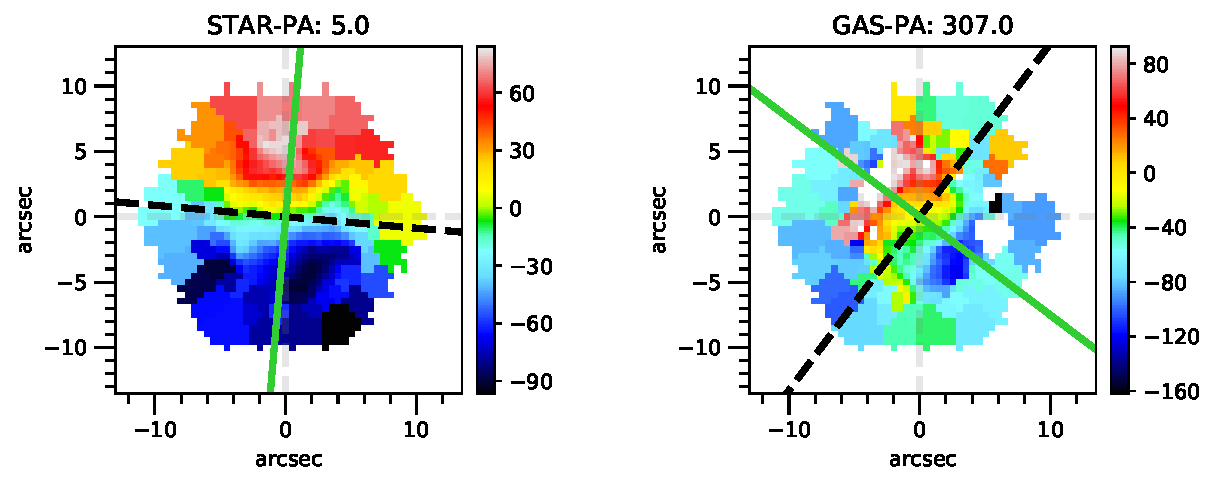
\includegraphics[width=0.8\textwidth]{images/PAplots/PAplotsCPSB/8313-6101-PA.pdf}
    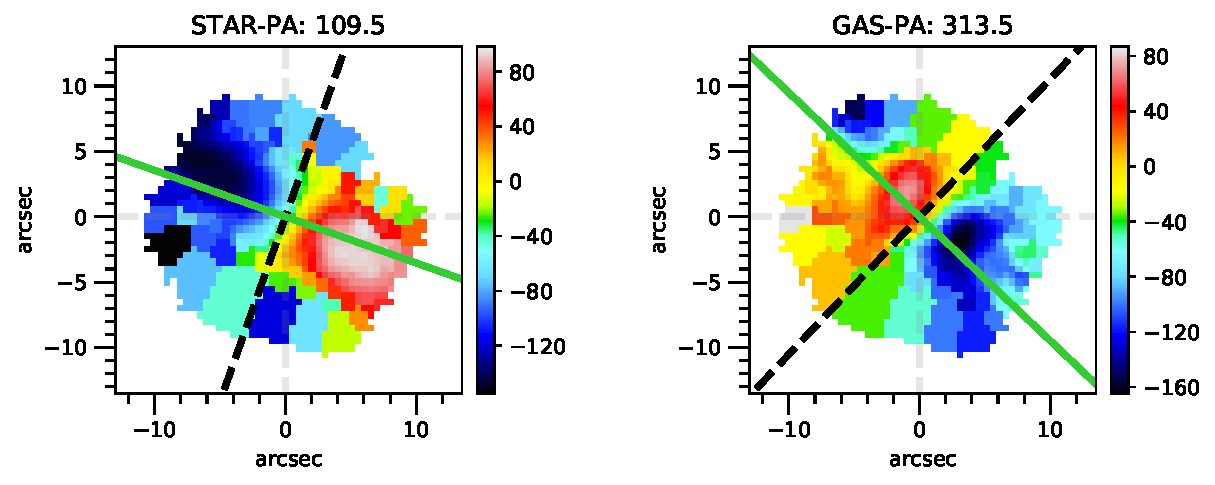
\includegraphics[width=0.8\textwidth]{images/PAplots/PAplotsRPSB/8323-6103-PA.pdf}
    \caption[Examples of PSBs showing significant kinematic PA misalignment $\Delta$PA$_{k}$]{Illustration of velocity field maps for PSBs with fitted kinematic position angles (PA$_{k}$) showing considerable misalignment. The stellar velocity fields (left) and gas velocity fields (right) are shown for CPSB 8313-6101 (top), and RPSB 8323-6103 (bottom). The position angles of the velocity field (gas or stars) are displayed as green solid lines, while the black dashed lines denotes the bisector of the velocity fields between the receding (red) and approaching (blue) sides. The velocity colour scale is \kms. Credit: Chris Duckworth.}
    \label{fig:CPSB-8313-6101-PA}
\end{figure*}


